\section{Mise en oeuvre d'un service de reconnaissance d'entités nommées}
Ayant les différents aspects de la mise en oeuvre d'un service de REN à l'Insee en tête, je m'attelle à la construction d'un service pérenne. Cela implique des choix d'architecture logicielle, à commencer par le choix de la bibliothèque de TLN.

\subsection{Stanford Core NLP ou SpaCy~: choix de la bibliothèque}

\subsubsection{Deux langages}
Choisir entre \textbf{SpaCy} et \textbf{Stanford Core NLP} implique de choisir entre le monde de \textbf{Java} et celui de \textbf{Python}. Plusieurs aspects sont à prendre en compte dans ce choix, à savoir la performance, la maintenabilité ainsi que la facilité de ré-utilisation. 
\newline

Tout d'abord la performance~: l'exécution d'un code Java nécessite d'abord sa compilation afin que le \textit{bytecode} qui en ressort soit interprété par la JVM~: \textit{Java Virtual Machine}. L'idée portée par le langage peut être résumé par la phrase suivante~: \textit{Write once, run everywhere}, compiler une fois, exécuter partout. Ce découpage implique un coût sur les performances des programmes Java. Ils ont tendance à consommer davantage de mémoire du fait que sa gestion est gérée uniquement par la JVM. Pour un programme ayant une grande utilisation de mémoire, ce qui est le cas en général pour les traitements NLP, le choix d'implémenter en Java a un impact. L'exécution d'un pipeline Stanford Core NLP nécessite en effet de donner au moins 2 Go de RAM à la JVM, afin notamment de monter en mémoire les paramètres des réseaux de neurones. L'utilisation conjointe du langage \textbf{Python} et du langage \textbf{Cpp}, via le compilateur \textbf{Cython} dans SpaCy, permet la gestion contrôlée de la mémoire. La bibliothèque tire partie des possibilités offertes par le Cpp également pour la parallélisation de tâches. Python est en effet un langage interprété~: il ne nécessite pas de compilation et est, comme pour un programme Java, interprété par un processus. L'interpréteur Python et son célèbre PIL pour \textit{Python Interpreter Lock} ne permet pas de faire du multi-threading et n'offre aucune gestion de mémoire. Il est davantage axé sur la lisibilité du code et donc sur sa maintenabilité, que le langage Java.
\newline

La différence de performance se fait sentir entre les deux bibliothèques. Pour l'analyse de deux textes, l'un étant une simple phrase, l'autre une publication de quatre pages, des différences notables de temps de calcul et d'occupation de mémoire sont observées. Le pipeline utilisé pour les tests exécute les traitements suivant~: \textit{Tokenization}, \textit{Sentence Split}, \textit{Part-of-Speech} et \textit{Dependencies}. Les ressources allouées sont de 0.4 CPU et 4 Go de RAM. La durée de l'initialisation est de trois à quatre secondes, pour Core NLP comme pour SpaCy. La durée de traitement est en revanche bien plus rapide avec SpaCy~: 200 millisecondes pour le premier exemple et moins de 600 pour le second. Core NLP traite lui le premier exemple en un peu plus d'une seconde et le second prend entre trois et quatre secondes. Concernant l'occupation mémoire des deux processus, elle est étonnamment équivalente~: 3.8 Go de RAM pour SpaCy comme pour Stanford Core NLP.

Des \textit{benchmarks}, tests sur des bases de données standards ayant pour vocation de faire référence sont disponibles sur la  \href{https://spacy.io/usage/facts-figures}{documentation de SpaCy} \cite{spacy-figures}.
\newline

Ensuite, la facilité de modification du code pour la maintenance est également un critère sur lequel les deux langages se distinguent. Le langage Java est verbeux~: le typage explicite, l'orientation «~tout objet~» et les nombreuses bibliothèques et outils utilisables offrent la possibilité de créer des programmes robustes et relativement tolérants aux changements. Le simple fait qu'il doit être compilé permet de détecter des erreurs avant l'exécution, là où un programme Python nécessite une exécution. Python a plusieurs avantages~: le langage est très permissif. Il permet de faire à la fois de la programmation orientée objet, de la programmation fonctionnelle et du \textit{scripting}. Cela s'adapte bien aux problématiques du \textit{Big Data}, où les données ont rarement un format homogène et où il est parfois difficile d'en faire une représentation objet. \textbf{SpaCy} permet par exemple l'ajout de champs à l'objet \textit{Doc} représentant le résultat d'un pipeline. Par ailleurs, le langage est très concis dans sa syntaxe. Ces deux derniers aspects du langage font d'un programme \textbf{Python} un programme simple à modifier, d'autant plus qu'il existe aujourd'hui énormément de bibliothèques \textit{Python} pour la Data Science et pour le Web.
\newline

Il y a enfin une dimension humaine à prendre en compte dans un tel choix, dans la perspective d'un développement à long terme. L'Insee a en effet acquis une bonne expertise dans les applications Java et R. Bien que le langage Python soit accessible, qu'il partage beaucoup de points communs avec le R, aucune application en Python n'est disponible en production à ce jour. Le langage est cependant très populaire auprès de la communauté et il est donc aisé de s'y former~:
\vspace{10pt}
\begin{figure}[H]
    \centering
    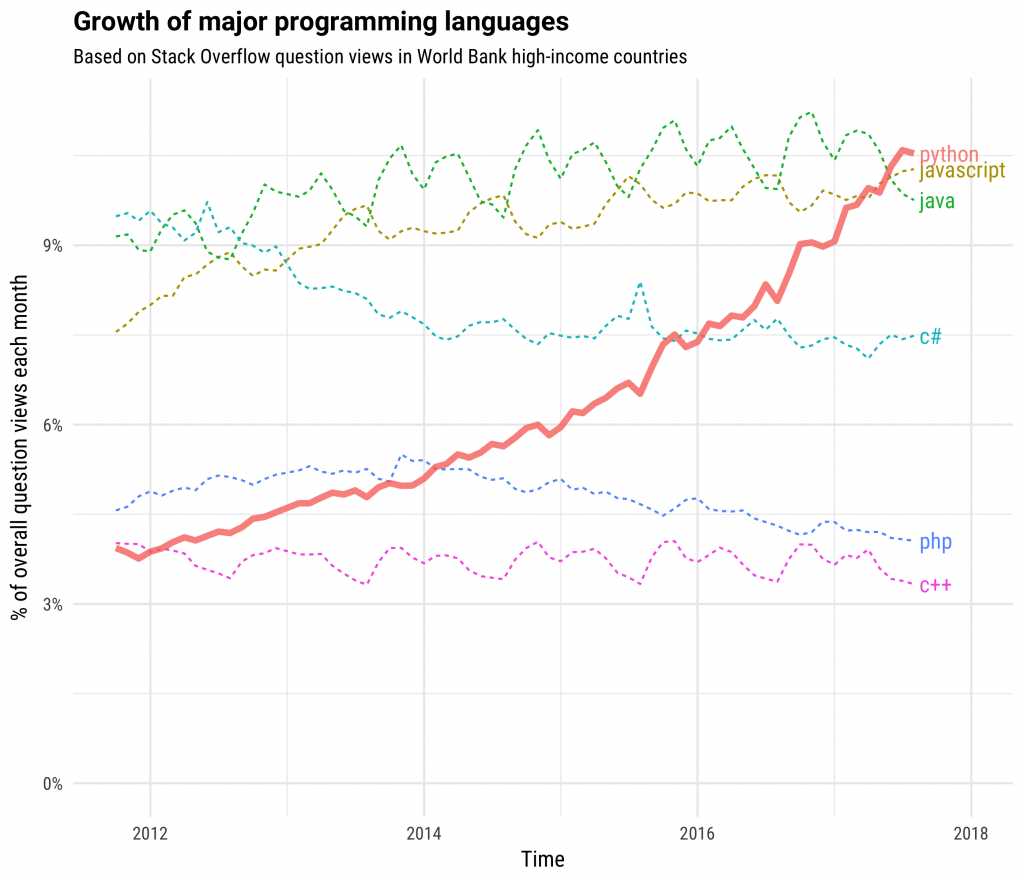
\includegraphics[scale=0.36]{images/languages-var.png}
    \caption{Évolution de la popularité des langages les plus utilisés entre 2012 et 2018}
    \label{fig:lang-var}
\end{figure}
\vspace{5pt}
Python a atteint une popularité semblable à Java ces dernières années, et semble conforter sa première place au classement de l'\textbf{IEEE}, devant Java.

Pour le langage, le bon choix technique semble être \textbf{Python} car les performances offertes par l'implémentation native de \textbf{SpaCy} sont bien meilleures que sur du Java, tout en ayant les avantages de Java. Le langage n'est évidemment pas le seul critère de distinction entre ces deux bibliothèques~: la fréquence de mises à jour, l'ouverture aux autres langues, la licence utilisée ou encore l'outillage autour du produit sont à prendre en compte.
\label{section 3.1.1}

\subsubsection{Deux philosophies}
Les buts recherchés derrière la création des deux bibliothèques sont différents~: Stanford Core NLP, dont la première version date de 2010, vise à montrer l'état de l'art dans le TLN. Elle rassemble beaucoup de fonctionnalités, essentiellement pour l'anglais et atteint de meilleures niveaux de précision que les bibliothèques standards. Le but d'\textbf{Explosion AI}, l'entreprise qui maintient \textbf{SpaCy}, est d'offrir un outil industriel facilement utilisable pour tous les cas d'applications~: ChatBot, corrections de formulaires, indexation de contenu, etc. La première version de la bibliothèque date de 2015. Elle est basée sur les travaux de recherches du groupe \textit{Stanford NLP}, et propose les fonctionnalités les plus génériques. \textbf{Explosion AI}, qui développe SpaCy, s'attache également à intégrer le plus de langues possibles, contrairement à Core NLP qui se concentre sur l'anglais.
\newline

Voici un tableau récapitulatif des différents traitements proposés par les bibliothèques~:
\vspace{10pt}
\begin{table}[H]
    \centering
    \begin{tabular}{| p{0.4\linewidth} | c | c | c |}
        \hline 
        \textbf{Fonctionnalités} &\textcolor{red}{Core NLP} &\textcolor{blue}{SpaCy} &\textcolor{orange}{NLTK}\\
        \hline
        \hline 
        \textit{Neural network models} &O &O &X\\
        \hline 
        \textit{Integrated word vectors} &X &O &X\\
        \hline 
        \textit{Multi-language support} &O &O &O\\
        \hline 
        \textit{Tokenization} &O &O &O\\
        \hline
        \textit{Part-of-speech tagging} &O &O &O\\		
        \hline 
        \textit{Sentence segmentation} &O &O &O\\
        \hline 
        \textit{Dependency parsing} &O &O &X\\
        \hline
        \textit{Lemmatization} &O &O &O\\
        \hline 
        \textit{Entity recognition} &O &O &O\\
        \hline 
        \textit{Entity linking} &O &X &X\\
        \hline 
        \textit{Coreference resolution} &O &X &X\\
        \hline 
        \textit{Open Information Extraction} &O &X &X\\
        \hline 
        \textit{Sentiment analysis} &O &X &X\\
        \hline
    \end{tabular}
    \caption{Tableau comparatifs des fonctionnalités proposées par les bibliothèques standards}
    \label{tab:nlp-compare}
\end{table}
\vspace{5pt}

Ce tableau est inspiré de celui proposé dans la \href{https://spacy.io/usage/facts-figures}{documentation de SpaCy} \cite{spacy-figures}; il le complète et le corrige avec l'état actuel des bibliothèques. NLTK, \textit{Natural Language Toolkit} est la bibliothèque historique de TLN en Python~: la première version date de 2001. En tant que référence de longue date dans le domaine du TLN, il est placé dans le tableau à titre de comparaison avec les autres bibliothèques.
\newline

Du fait de son orientation recherche, Core NLP offre davantage de fonctionnalités en anglais, notamment \textit{Entity Linking} et \textit{Coreference resolution} qui sont des traitements utiles dans notre cas d'utilisation. Ces fonctionnalités que n'a pas SpaCy sont assez dépendantes du contexte d'utilisation~: \textit{Entity Linking} dépend de la base de données utilisée. \textit{Open Information Extraction}, qui s'attache à extraire des triplets sujet-relation-objet d'un texte dépend de l'ontologie utilisée. Ces fonctionnalités ne sont donc pas réutilisables dans des contextes spécifiques, l'objectif de la bibliothèque étant de montrer que ces traitements sont possibles, et non de fournir un outil. C'est l'objectif affiché par SpaCy et c'est la raison pour laquelle elle intègre des dictionnaires de vecteurs de mots.
\newline

La différence entre les deux bibliothèques apparaît également dans la possibilité de personnaliser et d'adapter les fonctionnalités à nos besoins. D'une part, la documentation de SpaCy est plus fournie et plus facile d'utilisation que celle de Core NLP. Cette dernière ne détaille pas toutes les fonctionnalités de l'outil, mais fait davantage référence à des articles de recherche. Cela permet une meilleure compréhension des mécanismes utilisés dans le TLN, mais nécessite davantage de temps pour maîtriser l'utilisation de l'outil. De plus, elle offre  davantage de personnalisation, avec notamment un outil générique, \href{https://stanfordnlp.github.io/CoreNLP/tokensregex.html}{\textit{TokensregexAnnotator}} \cite{corenlp-tokensreg}, qui fournit un langage spécifique à la bibliothèque pour effectuer des traitements. L'outil équivalent de SpaCy, \href{https://spacy.io/usage/rule-based-matching}{\textit{Matcher}} \cite{spacy-ruler} n'est pas aussi générique et l'efficacité est préférée~: le format utilisé est standard (\textbf{jsonl}) et la grammaire reste simple.
\newline

Pour notre cas d'étude, deux aspects sont à étudier plus précisément~: la généralisation des traitements aux autres langues, la licence utilisée et les différences sur la reconnaissance d'entités nommées. La diversité des langues gérées par les bibliothèques est en effet importante dans la perspective de mutualisation des investissements Insee à l'échelle européenne (voir section \ref{section 2.1.4}). 
\label{section 3.1.2}

\subsubsection{L'ouverture du service}
Bien que le \autoref{tab:nlp-compare} montre un support multilingue des deux bibliothèques, il est à détailler. Le groupe de recherche de Stanford s'est en effet concentré sur la langue de Shakespeare, et offre des modèles pour l'Arabe, le Chinois, le Français, l'Allemand et l'Espagnol. De plus, ces modèles n'offrent pas toutes les fonctionnalités comme on peut le voir dans ce tableau issu de la \href{https://stanfordnlp.github.io/CoreNLP/human-languages.html}{documentation de Core NLP} \cite{corenlp-lang}~:
\vspace{10pt}
\begin{table}[H]
    \centering
    \begin{tabular}{| p{0.35\linewidth} | c | c | c | c | c | c |}
        \hline
        \textbf{Traitements} &AR &ZH &EN &FR &DE &ES\\
        \hline 
        \hline
        \textit{Tokenization} &O &O &O &O &X &O\\
        \hline
        \textit{Part-of-speech tagging} &O &O &O &O &O &O\\		
        \hline 
        \textit{Sentence segmentation} &O &O &O &O &O &O\\
        \hline 
        \textit{Dependency parsing} &X &O &O &O &O &X\\
        \hline
        \textit{Lemmatization} &X &X &O &X &X &X\\
        \hline 
        \textit{Entity recognition} &X &O &O &X &O &O\\
        \hline 
        \textit{Entity linking} &X &O &O &X &X &X\\
        \hline 
        \textit{Coreference resolution} &X &O &O &X &X &X\\
        \hline 
        \textit{Open Information Extraction} &X &X &O &X &X &X\\
        \hline 
        \textit{Sentiment analysis} &X &X &O &X &X &X\\
        \hline
    \end{tabular}
    \caption{Tableau récapitulatif des traitements de Core NLP en fonction de la langue}
    \label{tab:corenlp-lang}
\end{table}
\vspace{10pt}

Pour notre cas d'application, on s'intéresse d'abord au français, puis à l'anglais et aux autres langues européennes. La bibliothèque offre pour ces dernières le traitement de REN, excepté pour le français. Les quatre traitements proposés ont toutefois un potentiel via l'utilisation des \textit{Tokensregex}.
\newline

Bien que le projet soit OpenSource et disponible sur \href{https://github.com/stanfordnlp/CoreNLP}{Github} \cite{corenlp-repo}, les contributions extérieures sont moins nombreuses que sur \href{https://github.com/explosion/spaCy}{SpaCy} \cite{spacy-repo}. Explosion AI encourage vivement les contributions extérieures, notamment en ce qui concerne la prise en charge d'autres langues. La bibliothèque propose à ce jour un large choix de modèles entraînés, avec parfois plusieurs modèles par langues~:
 \vspace{10pt}
\begin{figure}[H]
    \centering
    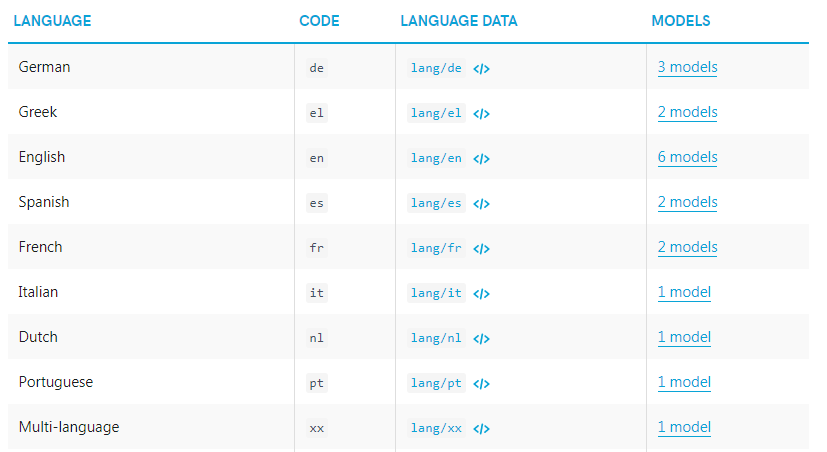
\includegraphics[scale=0.7]{images/spacy-lang.png}
    \caption{Tableau récapitulatif des modèles disponibles pour SpaCy, tiré de la \href{https://spacy.io/usage/models}{documentation}} \cite{spacy-lang}
    \label{fig:spacy-lang}
\end{figure}
\vspace{10pt}

Toutes les langues listées ci-dessus proposent les traitements de SpaCy listés \autoref{tab:nlp-compare}. Pour le modèle multilingue (ML), il propose uniquement la REN pour l'anglais, l'allemand, l'espagnol, le français, l'italien, le portugais et le russe. D'autres modèles sont à l'étude et utilisables~: ils couvrent plus d'une vingtaine de langues d'Asie et d'Europe. Les ajouts de supports de langues et autres mises à jours sont assez fréquents sur SpaCy. La communauté autour de l'outil est très active et de nombreuses améliorations apparaissent petit à petit. Comme on peut le voir sur le \href{https://github.com/explosion/spaCy}{Github} \cite{spacy-repo} du projet, toutes les améliorations, idées d'améliorations et bugs sont publiés. J'ai notamment eu l'occasion de proposer une idée d'amélioration pour le format de sortie des données. Les personnes qui maintiennent la bibliothèque semblent très réactifs et à l'écoute de la communauté, ce qui facilite à la fois la visibilité de la bibliothèque et son ouverture aux autres langues. A titre d'exemple, Explosion AI sort actuellement une mise à jour tous les un à deux mois. À titre de comparaison, la dernière mise à jour de Stanford Core NLP date d'octobre 2018.
\newline

N'ayant pas une grande expertise sur le TLN et sur les autres langues en général, le bon choix, afin de profiter d'une communauté active et de nouvelles fonctionnalités fiables, semble être SpaCy. Il reste  à aborder l'aspect central du projet~: la construction d'un pipeline de reconnaissance d'entités nommées.
\label{section 3.1.3}

%TODO : ajouter quelque chose sur la licence

\subsubsection{La REN dans les deux bibliothèques}
Bien que le sujet soit déjà abordé dans la partie \ref{section 2.2.4} avec Core NLP, certains points concernant la REN, notamment avec SpaCy, restent à aborder. 
\newline

SpaCy offre les mêmes fonctionnalités pour reconnaître ses propres entités nommées, à savoir la reconnaissance à base de règles et celle à base de réseaux de neurones. Pour les règles, SpaCy intègre un composant, \textit{EntityRuler}, qui permet de faire directement de la REN avec les règles, là où Core NLP est plus général avec les \textit{Tokensregex}. La syntaxe est plus simple avec SpaCy qui utilise un format standard (voir page \pageref{rule-exemple}).
\newline

La bibliothèque propose également deux modèles de REN, qui reconnaissent les entités de type personne, lieux, organisation et divers. Quelques rapides tests montrent que le modèle \textit{small} a ses limites, notamment sur le \textit{POS-tagging}, tandis que le modèle \textit{medium} reconnaît assez généralement les trois premiers types d'entités. Quasiment aucun concept statistique n'est reconnu en tant qu'entité diverse par le modèle. Un test a également été réalisé à partir d'un modèle de REN compatible avec Core NLP et entraîné par \href{http://lab.kbresearch.nl/static/html/eunews.html}{Europeana} \cite{europeana-ner}. % TODO : compléter
\newline

Là encore, SpaCy semble plus adapté pour construire un service de reconnaissance d'entités nommées, sa simplicité d'utilisation et son efficacité étant nettement meilleure que ce qui est proposé par Core NLP. C'est donc assez naturellement que \textbf{SpaCy} a été choisi pour construire le service. 
\label{section 3.1.4}

\subsection{L'architecture du projet}

\subsubsection{Une architecture micro-service}
Pour faciliter l'intégration avec d'autres services qui pourraient être développés ultérieurement (voir section \ref{section 2.1.4}), j'ai fait le choix de construire un web-service sous forme d'\textbf{API REST} qui effectue la REN. Il s'impose assez naturellement~: d'une part parce que c'est un standard du web, et d'autre part parce qu'il s'adapte parfaitement bien au cas d'usage.
\newline

L'objectif à court terme est de construire un service applicatif et un service utilisateur. Les deux services s'articulent comme suit~:
\vspace{10pt}
\begin{figure}[H]
    \centering
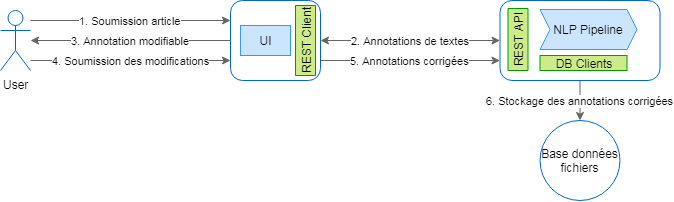
\includegraphics[scale=0.62]{images/Archi-pipeline-web.png}
    \caption{Articulation des Web-services à mettre en place}
    \label{fig:archi-pipeline-web}
\end{figure}
\vspace{10pt}

Ce choix d'architecture a été guidé par une réflexion sur les fonctionnalités assurées par le service. Ce dernier doit se concentrer principalement sur la REN, et non sur le format des données d'entrée/sortie. C'est pourquoi le format des données échangées doit rester simple et standard~: le choix s'est porté sur du \textbf{json}, \textit{JavaScript Object Notation}. Python propose en effet nativement des objets similaires ainsi que des bibliothèques associées très faciles d'utilisation. Bien qu'il soit incomplet, un résultat des traitements au format json est donnée par une fonction de la bibliothèque SpaCy. J'ai d'ailleurs soumis une \textit{issue} sur le \href{https://github.com/explosion/spaCy/issues/3987}{Github} \cite{spacy-issue} du projet SpaCy, qui propose d'améliorer ce rendu. Je n'ai à l'heure actuelle pas trouvé le temps de l'implémenter, cela nécessitant une connaissance approfondie de l'implémentation de la bibliothèque et de \textbf{Cython}.

Dans le cas d'une utilisation avec les publications de l'Insee, l'idée est de laisser la gestion du format des publications au service utilisateur, qui fait alors plusieurs appels au serveur applicatif pour annoter la totalité d'une publication. Cela permet de ne pas perdre les informations liées au format. Ce choix a de plus l'avantage de laisser le serveur applicatif sans état, \textit{stateless}, ce qui facilite la gestion de plusieurs instances et donc le passage à l'échelle. Cela est une qualité importante du Web-service~: les utilisations possibles, comme décrites section \ref{section 2.1.3} sont nombreuses et il est nécessaire de maintenir une bonne disponibilité. Cela est d'autant plus important que les traitements prennent du temps, environ quelques centaines de millisecondes~: le nombre d'instances à déployer peut donc vite augmenter.
\newline
\label{section 3.2.1}

\subsubsection*{Architecture des services}
L'architecture du service d'application ressemble au premier service décrit à la section \ref{section 2.2.5}. Elle intègre cependant quelques changements, notamment sur l'ajout des entités à reconnaître~:
\vspace{10pt}
\begin{figure}[H]
    \centering
    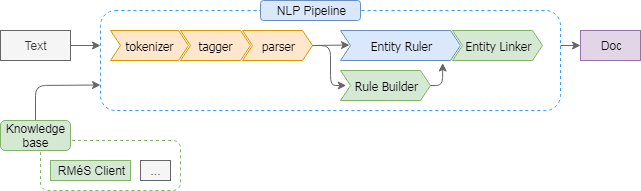
\includegraphics[scale=0.36]{images/InspaCy-archi.png}
    \caption{Architecture du service de REN}
    \label{fig:inspacy-archi}
\end{figure}
\vspace{10pt}

Dans le premier pipeline, l'ajout de nouvelles entités à reconnaître se faisait «~à la main~», c'est-à-dire en ajoutant une ligne au fichier des entités nommées. Dans l'architecture décrite ci-dessus, l'idée est de proposer une base de connaissance sous forme de clients de base de données. Ces clients récupèrent au lancement du programme les libellés et identifiants des entités nommées de leur base pour les traiter via un pipeline TLN et créer des règles. Quatre composants permettent de créer ces règles~: \textit{Tokenizer}, \textit{Tagger} et \textit{Parser}, dont les instances sont partagées avec le pipeline principal au lancement du serveur et le composant \textit{Rule Builder}. Ce dernier composant récupère l'annotation issue du pipeline pour créer les règles et les injecter directement dans le composant \textit{Entity Ruler}. Cela évite de stocker les règles sur le disque, comme cela est le cas avec le premier service.
Le second changement se situe au niveau du composant \textit{Entity Linker}. Bien qu'une \textit{issue} sur le dépôt \href{https://github.com/explosion/spaCy/issues}{Github} \cite{spacy-repo} semble indiquer que le composant est en cours d'implémentation, j'ai préféré en créer un moi-même afin de pouvoir avancer dans l'implémentation. Les traitements de reconnaissance et de ceux de liens avec des bases de données sont séparés dans ce pipeline, afin de pouvoir tester différentes bases de connaissances. Le cas des concepts géographiques en est un bon exemple.
\newline

La méthode de REN ne change pas dans ce service~: j'intègre toutefois la possibilité de générer des règles plus simples que celles décrites dans la section \ref{section 2.2.5}. Ces types de règles supplémentaires cherchent les libellés exacts, en prenant ou non en compte la casse. Cela a pour but de pouvoir ajouter facilement des entités plus spécifiques, comme des organisations (Ministères, Eurostat) ou encore des lieux. Bien que SpaCy propose des modèles de REN pour le français capables de reconnaître ces concepts, je fais le choix de ne pas les utiliser~: les composants \textit{Entity Ruler} et \textit{Entity Recognizer} fonctionnent mal ensemble (voir section \ref{section 3.1.4}). Cela implique nécessairement d'intégrer différents types de règles pour reconnaître d'autres types d'entités (nombres, noms propres). 
\newline

L'interface utilisateur doit permettre à un rédacteur d'obtenir un retour sur sa publication et d'éditer les annotations du service de REN. Il devra donc avoir un module à part pour gérer le format des publications. Voilà les fonctionnalités attendues~:
\vspace{5pt}
\begin{itemize}
    \item L'interface doit permettre d'entrer du texte directement sur la page ou de soumettre un fichier depuis le disque local. On doit pouvoir spécifier le format du fichier et sa grammaire associée. Pour le moment, un module pour le XML suffit.
    \vspace{5pt}
    \item À partir de la réponse du serveur REN, l'interface doit présenter le texte comme un ensemble de boutons, chaque bouton correspondant à un token. Ces boutons doivent être de couleurs différentes si ce sont des entités nommées (voir \href{https://spacy.io/usage/visualizers#ent}{displaCy}\cite{displacy}).
    \vspace{5pt}
    \item L'utilisateur doit pouvoir rassembler/désassembler les tokens pour les annoter en tant qu'entités nommées, ainsi que choisir le type d'entité nommée (Concept statistique, Organisation, Lieux, Dates).
    \newline
\end{itemize}

L'architecture des services web établie, il a fallu choisir les frameworks qui facilitaient l'implémentation des deux services.
\label{section 3.2.1 - Architecture des services}

\subsubsection{Les technologies utilisées}
Le choix s'est très vite fixé pour l'implémentation du service de REN sur \href{https://github.com/pallets/flask}{Flask} \cite{flask}. La facilité d'utilisation, la rapidité avec laquelle on peut mettre en place un service, tout en garantissant le passage en production, le framework est tout indiqué. Ayant peu de connaissances sur le développement web \textit{front-end}, il était difficile pour moi d'effectuer un choix de technologies pour l'interface. \textbf{Angular}, \textbf{React}, \textbf{Vue.js}, de nombreux frameworks Javascript existent et il n'est donc pas évident de se fixer sur un outil. J'ai à cet occasion été conseillé par Éric Sigaud de la DIIT (voir section \ref{section 1.1.2}) et Renaud Genevois de la Division Architecture Applicative de Production (DAAP), principal développeur d'\textit{Onyxia-IHM}. Cette dernière a été développée en React et j'ai pu explorer son code source.
\label{section 3.2.2}

\subsubsection*{Flask \& Python~: créer un web service en une heure}
La principale qualité de Flask et des frameworks Python en général est la rapidité avec laquelle on peut créer et déployer un web-service. Afin d'en faire un web-service, il a suffit d'ajouter un simple fichier Python décrivant les routes et méthodes HTTP associées. Comparativement à \textbf{JAX-RS}, framework standard Java pour mettre en place une API REST, ou encore à \textbf{Javalin}, plus récent, l'implémentation avec Flask est beaucoup plus légère. Là où les framework Java proposent des interfaces à implémenter, des annotations et des dépendances à choisir, Flask requiert une simple ligne de code et des décorateurs (équivalent des annotations Java).
\newline

Flask intègre également un outil de \textit{templating html}, \textbf{Jinja2}, qui permet de créer une petite interface web. J'ai donc pu intégrer rapidement une interface pour tester à la main le service. J'y ai ajouté pour le moment des options pour pouvoir aisément vérifier les résultats du pipeline. Ce framework se complète très bien avec \textbf{SpaCy}~: la bibliothèque TLN intègre depuis peu un outil fournissant un visuel HTML pour les résultats de REN et de dépendances. Cela permet avec Jinja2 une intégration du rendu généré par le module \textbf{displacy} directement dans la page HTML. C'est là encore une illustration de la rapidité avec laquelle on peut mettre en place un web-service avec \textbf{SpaCy} et \textbf{Flask}. Voilà un aperçu de la page de démonstration réalisée avec ces deux outils~:
\begin{figure}[H]
    \centering
    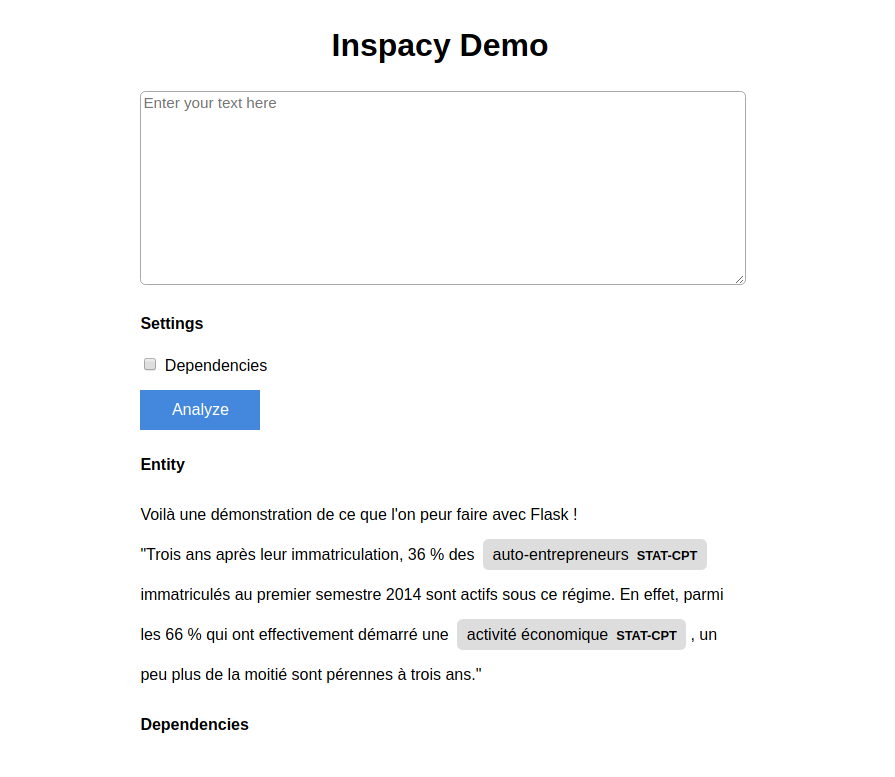
\includegraphics[scale=0.6]{images/inspaCy-demo.png}
    \caption{Capture du service de reconnaissance d'entités nommées développé avec Flask}
    \label{fig:demo-inspaCy}
\end{figure}

J'ai pu grâce à Flask, mettre en place le web service en une journée~: création des routes, formatage des données et interface minimaliste. Cela rejoint l'analyse des différences relevées entre Python et Java section \ref{section 3.1.1}~: Python est très efficace pour prototyper et tester, sans avoir à se soucier d'aspects bas niveau comme la gestion de la mémoire, les entrés-sorties ou encore la gestion des dépendances.
\label{section 3.2.2 - Flask}

\subsubsection*{React}
Le choix pour l'interface utilisateur s'est finalement porté sur React. Framework Javascript le plus populaire actuellement, comme le montre cet article de \href{https://stackoverflow.blog/2018/01/11/brutal-lifecycle-javascript-frameworks/}{stackoverflow} \cite{stackoverflow-javascript}, il permet de créer une interface utilisateur sous forme de composants. Utilisant un DOM virtuel, \textit{Document Object Model}, il permet d'intégrer des composants complexes dans une interface, et ce de façon dynamique. Développer une interface consiste donc simplement à placer des composants et à créer les fonctions définissant les comportements spécifiques au cas d'usage. De nombreuses bibliothèques de composants React existent à ce jour (\textbf{Material-UI}, \textbf{React-bootstrap}, \textbf{React toolbox}, etc.), offrant toutes sortes de boutons, menus et éléments d'interactions. N'ayant jamais développé de projet en Javascript, cela m'a permis en très peu de temps de faire une petite interface pour un projet associatif.
% TODO : trouver une meilleure ref pour React.
\newline

J'ai cependant manqué de temps pour obtenir une interface fonctionnelle, que ce soit pour mon projet associatif ou pour l'interface utilisateur. Bien que Javascript soit assez accessible pour quelqu'un ayant développé dans d'autres langages, le framework React nécessite une connaissance approfondie du développement \textit{Front-end}~: gestion du cache, appels asynchrones à une API ou encore découpage de l'application en composants, il me reste encore beaucoup de choses à apprendre sur \textbf{React} pour être efficace sur le développement d'une interface utilisateur. Ne disposant pas du temps suffisant pour développer l'interface, et dans la mesure où l'Insee dispose d'agents maîtrisant le framework, je me suis donc contenté de laisser les spécifications.
\newline

Motivé et éclairé par le pipeline mis en place pour le premier service de REN, j'ai pu pour ce second programme apprécier les outils de la plateforme Innovation qui m'ont permis de développer en continu.
\label{section 3.2.2 - React}

\subsubsection{Intégration dans la démarche DevOps}
Tests, mise en service et déploiement de l'application~: j'ai voulu cette fois-ci automatiser tout le processus de vie du web-service, jusqu'à un déploiement sur la plateforme innovation. Je me suis cependant très vite heurté à un problème majeur~: la bibliothèque \textbf{SpaCy} n'est pas compatible avec le poste sur lequel je travaille. Manquant de temps, je me suis rapidement adapté en travaillant sur mon ordinateur personnel. N'étant pas relié au réseau, il est difficile d'accéder au \textbf{GitLab} et de manière générale à la plateforme Innovation. J'ai donc travaillé sur \textbf{Github}, et effectué un lien manuel avec GitLab à partir de mon poste de travail. \textbf{Git} étant un mécanisme de versionnement non centralisé, il permet d'avoir plusieurs dépôts distants~: dans le cas du dépôt de mon poste de travail, un dépôt Github et un dépôt GitLab. Dans l'idéal, il aurait fallu intégrer un \textit{web hook} sur Github, afin que chaque mise à jour du dépôt lance le pipeline CI/CD sur le dépôt GitLab. \textbf{Github Action} fournit un outil spécifique pour lancer des jobs sur un GitLab depuis un dépôt Github.
\newline

Bien que je n'aie pas eu le temps de mettre en place le processus d'intégration et de déploiement en continu, j'ai préparé le terrain~: afin d'effectuer le deploiement sur la plateforme innovation, il est nécessaire d'ajouter au projet plusieurs fichiers~:
\vspace{5pt}
\begin{itemize}
    \item Une image Docker~: c'est l'environnement d'exécution de l'application. Pour l'immense majorité des services, cet environnement est basé sur une distribution linux légère, auquel on ajoute les dépendances dont a besoin l'application pour s'exécuter correctement. Dans le cas du service de REN, on a donc besoin d'un environnement contenant \textbf{Python 3.6} ou toute version ultérieure, ainsi que les bibliothèques \textbf{Python} utilisées dans le projet (SpaCy, Flask, Flask-CORS, requests). Le choix est fait d'intégrer ces bibliothèques directement dans l'image, plutôt que de les télécharger à chaque lancement du conteneur~: cela augmente le volume de l'image Docker mais permet de gagner en rapidité de lancement du conteneur. SpaCy est en effet assez lourd et nécessite de plus les modèles de TLN, qui sont eux aussi volumineux. J'ai donc pris le temps de construire cette image Docker afin de faciliter l'avancement futur du projet.
    \vspace{5pt}
    \item Un contrat de déploiement~: il spécifie comment le conteneur doit être déployé sur la plateforme. Ressources à allouer, ports à exposer, réseau Docker sur lequel le déployer ou encore variables d'environnements à ajouter~: toutes ces informations sont données à \textbf{Marathon} qui déploie le service sur un nœud du cluster. 
    \vspace{5pt}
    \item Le fichier décrivant le pipeline~: \textit{.gitlab-ci.yml} pour GitLab, il spécifie les étapes du pipeline, les environnements à utiliser et les commandes shell à exécuter.
    \newline
\end{itemize}

J'ai donc préparé au mieux la mise en place d'un pipeline de déploiement continu, afin de faciliter l'intégration d'autres fonctionnalités, telles que l'ajout d'entités nommées ou l'ajout d'un client \textbf{Minio} pour stocker les données d'entraînement. Une évaluation des données d'entraînement est également à l'étude, afin de savoir si l'on peut lancer un entraînement.
\label{section 3.2.3}

\subsubsection*{Conclusion}
Le développement de ce service, de la méthode à la mise en service, m'a beaucoup apporté sur la mise en production d'applications. Tant sur les choix d'outils que sur les choix d'architecture, j'ai eu l'occasion de mobiliser les compétences acquises dans ma formation, et plus particulièrement dans mon projet de fin d'étude.
